\begin{chapter}{\label{cha:theoretical_model}Theoretical Modelling of Bose-Einstein Condensates}
\section{\label{section:meanfield} Mean-field description}
We aim to accurately model the dynamics of a closed system containing a dilute, weakly interacting Bose gas of $N$ atoms, at extremely low temperature. One could model the entire system by constructing a N-body quantum wavefunction, which would follow the Schr\"odinger equation, but the complexity of this method makes it extremely unwieldy to model the large number of particles used in Bose-Einstein condensate (BEC) experiments.

We instead model the system with a mean-field theory, described in Section \ref{section:gpe}, in which there are essentially two main approximations. First, justified by the dilute property of the gas, any binary interaction between particles at $\mathbf{r}$ and $\mathbf{r}'$ is assumed to be a contact interaction following a delta function of the form
\begin{equation*}
V(\mathbf{r}-\mathbf{r}') = g \delta(\mathbf{r}-\mathbf{r}'),
\end{equation*}
where $g$ is an interaction coefficient. Interactions involving a higher number of particles are ignored. Secondly, we assume that all particles in the condensate are macroscopically described by a single wavefunction, $\psi(\mathbf{r},t)$, where $\mathbf{r}$ is position and $t$ is time. As the particles all share the same phase and quantum state, $\psi(\mathbf{r},t)$ is a classical field. This second approximation also assumes that there are no particles contributing to thermal or quantum fluctuations beyond the classical field, and so is only justified in general in the limit of zero temperature. Nevertheless, we go further and describe some finite-temperature based effects in Sections \ref{section:dgpe}
and \ref{section:cfield}.

\section{\label{section:gpe} The Gross-Pitaevskii equation}
The result of the mean-field methodology is the Gross-Pitaevskii equation (GPE), 
\begin{equation}
i \hbar \frac{\partial\psi({\bf r},t)}{\partial t} = \left(-\frac{\hbar^2}{2m}\nabla^2 + V({\bf r},t) + g|\psi({\bf r},t)|^2 - \mu \right) \psi({\bf r},t),
\label{eq:gpe}
\end{equation}
where $m$ is the mass of a single particle, $\mu$ is the chemical potential, and $V({\bf r},t) = V_{\mathrm{obj}}({\bf r},t) + V_{\mathrm{trap}}({\bf r},t)$ is an external potential. In the case of no obstacles or surfaces the obstacle potential is $V_{\mathrm{obj}}({\bf r},t)=0$, otherwise $V_{\mathrm{obj}}({\bf r},t)$ is defined using Gaussian or step functions, as shown in Section \ref{section:potentials}. In the homogeneous case the trapping potential is $V_{\mathrm{trap}}({\bf r},t)=0$, otherwise harmonic trapping is used, such as $V_{\mathrm{trap}}({\bf r},t)=m\omega{\bf r}^2/2$ for a 3D spherically symmetric trap.

The GPE takes the form of a non-linear time-dependent Schr\"odinger equation, where the first two terms on the right hand side are the energy of a single particle in a potential field, and the third non-linear term describes the interactions between the multiple particles in the system, with a strength usually parametrised by $g=4\pi\hbar^2a/m$,
where $a_s$ is the s-wave scattering length. The wavefunction of the system is normalised so that the integrated density is equal to the number of atoms $N$,
\begin{equation}
\int\!|\psi|^2\,{\rm d}^3{\bf r} = N.
\label{eq:normalisewf}
\end{equation}

Taking into account the fact that the GPE is only strictly valid at $T=0$, it turns out the equation is surprisingly successful at quantitatively modelling ultra-cold gasses, even up to a temperature of $T\simeq T_c/2$, where $T_c$ is the critical temperature for Bose-Einstein condensation \cite{Proukakis}. The GPE also provides a qualitative model of BEC based effects in superfluids such as liquid helium II \cite{RobertsBerloff} and rotating neutron star cores \cite{Warszawski01082011}.

A detailed explanation of the mean-field formulation of the model and the full derivation of the GPE is shown in Section \ref{appsection:gpeqft}.

\section{\label{section:gpestationary} Time-independent Gross-Pitaevskii equation}
 We find a stationary version of the GPE by first fixing the potential, $V({\bf r})$, so that it is constant in time, and then writing the wavefunction in the form $\psi({\bf r},t) = \psi_0({\bf r})$, where $\psi_0({\bf r})$ is a stationary state. Equation \ref{eq:gpe} then becomes
	\begin{equation}\label{eq:stationgpe}
		\mu\psi_0({\bf r}) = \left( -\frac{\hbar^2}{2m}\nabla^2 + V({\bf r}) + g|\psi_0({\bf r})|^2  \right) \psi_0({\bf r}),
	\end{equation}
	the time-independent GPE. In the absence of interactions, $g=0$, this reduces to the standard time-independent Schr\"odinger equation, with the chemical potential $\mu$ reducing to the energy per particle. This version of the GPE can be used to find stationary solutions of the system, with the value of $\mu$ characterising the energy of the ground state.

\section{\label{section:mu} The chemical potential}
 The chemical potential of the system, $\mu$, can be thought of as the energy required to remove a particle from a system with large $N$, or alternatively as a measure of the energy of a particle. The value of $\mu$ will vary for the specific species of bosons considered and provides a useful scale of energy.
 
 The chemical potential can be found in terms of energies of the system by direct integration of Equation \ref{eq:stationgpe},
 	\begin{equation}\label{eq:chempot}
 		\mu = \left ( E_{\mathrm{kin}} + E_{\mathrm{pot}} + 2E_{\mathrm{int}} \right ) / N,
 	\end{equation}
 	where the quantities $E_{\mathrm{kin}}$, $E_{\mathrm{pot}}$ and $E_{\mathrm{int}}$ are defined in Appendix \ref{appsection:energy}.

\section{\label{section:quasi2dgpe} Quasi-two-dimensional Gross-Pitaevskii equation}
	For some condensate geometries it is useful to be able simulate the condensate via a lower dimensional GPE. An example of this is a highly oblate condensate, in which the trapping potential is defined as
	\begin{equation}
		V_{\mathrm{trap}}(x,y,z)=m\omega_\perp^2\frac{\left ( x^2+y^2 \right )}{2} + m\omega_z^2\frac{z^2}{2},
	\end{equation}
	with trapping frequencies $\omega_z \gg \omega_\perp$ and under the condition $\hbar\omega_z \gg \mu$, where $\mu$ is the 3D chemical potential. Tight $z$ confinement causes the dynamics to become essentially two dimensional (experimentally achieved in \cite{Gorlitz}) as the wavefunction along $z$ becomes fixed into the time-independent harmonic oscillator ground state, $\psi_z(z)$, so that
	\begin{equation}
		\psi({\bf r},t) = \psi_\perp(x,y,t) \psi_z(z),
	\end{equation}
	where $\int\!|\psi_\perp|^2\,{\rm d}^2{\bf r} = N$ and $\int\!|\psi_z|^2\,{\rm d}z = 1$ by convention. An expression for $\psi_z$ is found by assuming a Gaussian ground state,
	\begin{equation}
		\psi_z(z) = \pi^{-1/4} l_z^{-1/2} \exp\left(-z^2/2l_z^2\right),
	\end{equation}
  where $l_z=\sqrt{\hbar/m \omega_z}$. This is known as the quasi-2D regime and when this form of $\psi$ is substituted into Equation \ref{eq:gpe} it forms a 2D GPE that can be used to model the system with reduced dimensionality, with the modified interaction term $g_{\mathrm{2D}} = g/( \sqrt{2\pi}l_z)$ \cite{parkerthesis}. The 3D chemical potential $\mu$ is also modified as an extra term is absorbed, $\mu_\mathrm{2D} = \mu - \hbar\omega_z/2$, and all other three-dimensional properties become two-dimensional.

	A similar process can be performed with `cigar' quasi-1D geometries so that a 1D GPE can be used with a modified $g_{\mathrm{1D}}$ interaction term, and $\mu_{\mathrm{1D}}$ chemical potential. As before all 3D properties become 1D, however as we will not consider quasi-1D regimes in detail, the specifics are omitted from this thesis.

\section{\label{section:hydrodynamic} Hydrodynamic interpretation}
	Often it can be helpful to write the GPE, via the so called Madelung transformation, as a set of hydrodynamic equations. The transformation reinterprets the wavefunction $\psi$ as a magnitude directly related to the fluid density and a phase which is directly related to the fluid velocity. We write the wavefunction in the form
	\begin{equation}
		\psi({\bf r},t) = R({\bf r},t)\exp (i\theta({\bf r},t)),
	\end{equation}
	 and identify the fluid density as $\rho=mR^2$ and the velocity as $\mathbf{v} = \hbar\nabla\theta/m $.
	In vector form we obtain a continuity equation
	\begin{equation}
	  \frac{\partial \rho}{\partial t} + \nabla\cdot(\rho{\bf v}) = 0,
	  \label{eq:MTcont}
	\end{equation}
	and an equation similar to the Euler equation for an inviscid fluid,
	\begin{equation}
	\rho\left( \frac{\partial \mathbf{v}}{\partial t} + \left( \mathbf{v} \cdot \nabla \right)\mathbf{v} \right) = -\nabla p - \nabla \mathbf{P} - \rho \nabla \left(\frac{V}{m}\right).
	\end{equation}
	where $P_{jk} = -\frac{\hbar^2}{4m^2}\rho\frac{\partial^2\ln{\rho}}{\partial x_j \partial x_k}$ is known as the quantum pressure.
	A detailed derivation of this result can be found in Appendix \ref{appsection:madtrans}.

\section{\label{section:quantisedcirculation} Quantised circulation}
An interesting feature of the GPE is that the fluid circulation must be quantised. We can see this by first writing the integrated change of phase along any closed curve $C$,
\begin{equation}
	\Delta\theta = \oint_C \! \nabla \theta  \, \mathrm{d}\mathbf{l},
\end{equation}
where $\mathrm{d}\mathbf{l}$ is the line element along $C$. The wavefunction at the start and the end of the integration must be single valued, so
\begin{equation}
	\exp (i\theta_0) = \exp (i\theta_0)\exp (i\Delta\theta),
\end{equation}
for some $\theta_0$. This is only satisfied when $\Delta\theta = 2\pi q$, with $q\in\mathbb{Z}$. Our local velocity is $\mathbf{v} = \hbar\nabla\theta/m $ and so we can write
\begin{equation}
	\Gamma = \oint_C \! \mathbf{v} \cdot \mathrm{d}\mathbf{l} = \frac{2 \pi \hbar}{m}q.
\end{equation}
Notice that we are now taking the line integral of the velocity; we have a formula for the circulation. We find the circulation must be quantised in units of $\kappa = 2 \pi \hbar/m$, the so called `quantum of circulation'. This is in stark contrast to classical fluids where the circulation can take any real value.

\section{\label{section:gpedimless} Dimensionless Gross-Pitaevskii equations}
	%Bose-Einstein condensates can be formed with almost any size or scale. A trapped atomic cold gas BEC in particular can be experimentally realised with a wide range of topologies and atom interaction strength. A wide range of parameters can be fairly easily manipulated with magnetic or optical potentials and Feshbach resonances [CITE]. Superfluid helium can also form in various sizes, with vortex core radii of $\sim$1 or $\sim$100 angstroms, depending on the isotope of helium used. The cores of neutron stars are even theorised to be superfluid on a large scale.
	Systems which exhibit superfluidity due to the phenomenon of Bose-Einstein condensation can form at almost any scale, from ultra-cold atomic BECs formed at the micron scale, % to meter scale vats of superfluid $^4He$ with vortex core radii of $\approx\! 1~\AA$ \cite{Rayfield1964},
	to containers of superfluid helium on the metre scale, to neutron stars, the cores of which are theorised to be superfluid on the kilometre scale \cite{Warszawski01082011}.

	A trapped atomic BEC in particular can be experimentally realised with a wide range of variable parameters and anisotropic geometries. Through creative use of magnetic or optical potentials, atomic BECs have been realised in toroidal ring \cite{persistent,Ramanathan11}, box-like \cite{gaunt_2013,chomaz_2015}, quasi-2D `pancake' \cite{Neely}, and quasi-1D `cigar' \cite{Burger99,Weller08} traps. Through laser `painting', a method to produce arbitrary and dynamic trapping potentials has even been demonstrated \cite{Henderson09}. Adding an additional dimension to the parameter space, Feshbach resonances can be used to realise atomic condensates over a wide range of both attractive and repulsive atom-atom interactions \cite{Inouye1998}.

	For these reasons it is desirable to rescale the quantities used in the GPE so that any of the calculations performed can be easily reformulated into any scale and parameter regime desired. We make this process easier by doing all calculations with dimensionless parameters. Another advantage of the dimensionless formulation is that the size of the values involved are all normalised on the scale of unity, reducing the chance of errors in numerical computation due to the floating point representation used by modern computer architectures.
	We present two methods of making the GPE dimensionless, the specific scaling used is chosen by the needs of the simulation and is usually apparent (such as by whether a trapping potential is involved).

	\subsection{\label{section:gpedimlesshomg} Homogeneous GPE}
		Consider an infinite and homogeneous system with repulsive interactions and where $V_{\mathrm{trap}} = 0$. In this system's ground state, $\psi$ does not depend on ${\bf r}$ or $t$, and so we can set the time and spatial derivatives in the GPE to zero,
		\begin{equation}
		0 = \left(g|\psi({\bf r},t)|^2 - \mu \right) \psi({\bf r},t).
		\end{equation}
		By rearranging, we can easily find the natural homogeneous density of the system: $\rho = |\psi|^2 = \mu/g$. We then choose to rescale the wavefunction using this value, so that $\bar{\psi} = \psi/\sqrt{\rho}$.

		By dimensional arguments (see Appendix \ref{section:healing} for details), the length scale of space is the healing length, $\xi = \hbar/\sqrt{mg\rho}$, and the length scale of time $\tau = \hbar/(g\rho)$. These units are often called the `natural units'. We define the rescaled dimensionless quantities as
		\begin{equation}
			\bar{t} = \frac{t}{\tau}, ~~~ \bar{r} = \frac{r}{\xi}, ~~~ \bar{\varepsilon} = \frac{\varepsilon}{\mu},
		\end{equation}
		for time, length, and energy respectively, where a tilde denotes a dimensionless quantity. Substituting the dimensionless quantities into Equation \ref{eq:gpe} leads to the homogeneous GPE,
		\begin{equation}\label{eq:dimgpehomg}
		i\frac{\partial\bar{\psi}({\bar{\bf r}},\bar{t})}{\partial {\bar{t}}} = \left( -\frac{1}{2}\bar{\nabla}^2 + |\bar{\psi}({\bar{\bf r}},\bar{t})|^2 + \bar{V}_{\mathrm{obj}}({\bar{\bf r}},\bar{t}) - 1 \right) \bar{\psi}({\bar{\bf r}},\bar{t}).
		\end{equation}
		The resulting normalisation condition for $\bar{\psi}$ is
		\begin{equation}\label{eq:intwfhomg}
			\int \! |\bar{\psi}|^2 \, \mathrm{d}^3\bar{\bf r} = 1.
		\end{equation}

	\subsection{\label{section:gpedimlesstrap} Trapped GPE}
		When considering a harmonically trapped condensate it is convenient to work with a wavefunction scaled so that the normalisation condition is similar to Equation (\ref{eq:intwfhomg}). We denote the scaled wavefunction for a harmonically trapped condensate $\tilde{\psi}$ and write
		\begin{equation}\label{eq:intwf}
			\int \! |\tilde{\psi}|^2 \, \mathrm{d}^3{\bf r} = 1.
		\end{equation}
		We introduce the harmonic oscillator length, $l_r = \sqrt{\hbar/(m\omega)}$, where $\omega$ is a trap frequency. This leads to the dimensionless rescalings,
		\begin{equation}
			\tilde{t} = t\omega, ~~~ \tilde{r} = \frac{r}{l_r}, ~~~ \tilde{\varepsilon}= \frac{\varepsilon}{\hbar\omega},
		\end{equation}
		for time, length, and energy respectively, where an overbar denotes a dimensionless quantity.
		We rewrite Equation \ref{eq:normalisewf} with dimensionless length to find,
		\begin{equation}
			\int \! |\psi|^2 \, \mathrm{d}^3{\bf r} = N \Rightarrow \int \! |\psi|^2 N^{-1} l_r^3 \, \mathrm{d}^3\tilde{\bf r} = 1,
		\end{equation}
		and so we rescale the wavefunction to satisfy Equation \ref{eq:intwf},
		\begin{equation}
			 |\tilde{\psi}|^2 = |\psi|^2 N^{-1} l_r^3 \Rightarrow \tilde{\psi} = \psi N^{-\frac{1}{2}} l_r^\frac{3}{2}.
		\end{equation}
	Substituting the new rescaled quantities into Equation \ref{eq:gpe} leads us to the trapped GPE,
	\begin{equation}\label{eq:dimgpetrapped}
		i\frac{\partial\tilde{\psi}({\tilde{\bf r}},\tilde{t})}{\partial {\tilde{t}}} = \left( -\frac{1}{2}\tilde{\nabla}^2 + \tilde{g}|\tilde{\psi}({\tilde{\bf r}},\tilde{t})|^2 + \tilde{V}({\tilde{\bf r}},\tilde{t}) - \tilde{\mu} \right) \tilde{\psi}({\tilde{\bf r}},\tilde{t}).
	\end{equation}
	where
	\begin{equation}
		 \tilde{g} = \frac{gN}{\hbar \omega l_r^3}.
	\end{equation}
\section{\label{section:imagTime} The imaginary time propagation method}
Many numerical explorations of quantum systems, particularly those associated with magnetic or optical trapping,  involve calculating the ground-state as either the final result or as a stepping stone for further calculations. While often there exists analytic solutions for a condensate ground state, this problem is often solved numerically using so called eigensolvers. Numerically finding the ground state becomes practically necessary if a simulation requires complicated potential fields.

There are several methods available for implementing a numerical eigensolver: inverse iteration and Lanczos methods \cite{thijssen1999computational}, systematic variational techniques \cite{Bao2003230}, boundary eigenvalue methods \cite{Edwards95}, conjugate gradient techniques \cite{NumericalRecipes} and imaginary time propagation \cite{PhysRevE.62.7438}. We choose to use the last of these methods due to its relative simplicity at the expense of computational time.

The imaginary time method revolves around moving from real to imaginary time using the substitution $t_i = -it$. This transforms the GPE into a form similar to a diffusion equation. As a result, a local equilibrium can be found by propagating in time. This can be understood by considering a solution of the form $\psi(\mathbf{r},t) = \sum_n \psi_n(\mathbf{r})\exp(-i E_n t/\hbar)$, where $\psi(\mathbf{r},t)$ is a superposition of eigenfunctions $\psi_n(\mathbf{r})$ with eigenvalues $E_n$. Under propagation of the GPE in imaginary time, the wavefunction exponentially decays,
\begin{equation*}
\psi(\mathbf{r},t_i) = \sum_n \psi_n(\mathbf{r})\exp\left(\frac{-E_n t}{\hbar}\right).
\end{equation*}
In particular, the decay rate is directly related to the size of the eigenvalues $E_n$, so that the contributions from higher energy eigenfunctions decay the fastest. The final ingredient is to inhibit the overall decay of the wavefunction by renormalising during propagation. After a sufficient transient time the contributions from higher energy eigenfunctions become negligible, forcing the wavefunction to tend towards the ground state.

The imaginary time propagation method converges on the ground state solution very slowly and so we must perform many numerical steps to prepare an initial state. A silver lining of this drawback is that the method can be used to prepare almost any viable initial state. For example, an initial condition consisting of a Thomas-Fermi profile with many vortices can be made more accurate with this method by imposing the phase during imaginary time propagation. The result is a less violent start to condensate dynamics; minimal sound is produced due to the difference between the approximate initial condition and a true solution of the GPE.

The energy can be used as a way to gauge the solution convergence. An example ground state solution for a 2D condensate in a harmonic trap is found using the imaginary time method and is shown with the energy in Figure \ref{fig_imagtimesolgs}. For $t_i > 0.6/\omega$ the computed ground state energy does not significantly change, a good indicator that the ground state has been found to sufficient accuracy.
\begin{figure}[!ht]
	\centering
   \begin{tikzpicture}
    \begin{axis}[
        width=0.6\linewidth,
        height=0.33\linewidth,
        xlabel=$t_i \omega$,
        ylabel=$E/(\hbar\omega)$,
        restrict x to domain=0:1,
        colormap name=hsvcl,
        major tick length = 0.07cm
      ]
      \addplot gnuplot [raw gnuplot,mark=none,color=black,thick]{
      	plot "numerics/figures/imag-time-prop-energy.txt" using 2:3 with lines;
      };
    \end{axis}
  \end{tikzpicture}
  \hspace{0.04\linewidth}
  \begin{tikzpicture}
  \begin{axis}[
    width=0.33\linewidth,
    height=0.33\linewidth,
    axis on top,
    xmin=-9,
    xmax=9,
    xlabel={$x/l_r$},
    ymin=-9,
    ymax=9,
    ylabel={$y/l_r$},
    major tick length = 0.07cm]

  \addplot graphics [xmin=-12.8,xmax=12.8,ymin=-12.8,ymax=12.8] {numerics/figures/imag-time-gs.png};
  \end{axis}
\end{tikzpicture}
	\caption{An example of the use of the imaginary time propagation method for finding the condensate ground state for a condensate with interaction energy $\tilde{g}=2000$ and $\tilde{\mu}=25.27$, with the Thomas-Fermi solution as the initial state. The density of the final ground state solution is shown (right) along with the energy of the solution as the method propagates through imaginary time (left).}\label{fig_imagtimesolgs}
\end{figure}

\section{\label{section:movframe} Transforming the reference frame}
	\subsection{\label{section:linearmovframe} Linearly translating frame to simulate flow}
	The GPE is transformed into the translating reference frame via the linear momentum operator. In quantum mechanics the momentum operator is defined in position space as $\hat{P} = -i\hbar\nabla$. In most cases we wish to translate the frame in order to simulate a flow and so the operator is rewritten so that the momentum is along a single axis (usually the $x$ axis),
	\begin{equation*}
	\hat{P}_x = -i\hbar\frac{\partial}{\partial x}.
	\end{equation*}
	This term can be added to the right hand side of the GPE to modify it such that it is in the reference frame moving along $x$. For example, the GPE in the frame translating along the $x$ direction with velocity $v$ is written,
	\begin{equation}\label{eq:linearframegpe}
	i\hbar \frac{\partial\psi({\bf r},t)}{\partial t} = \left(-\frac{\hbar^2}{2m}\nabla^2 + V({\bf r},t) + g|\psi({\bf r},t)|^2 - \mu -vi\hbar\frac{\partial}{\partial x} \right ) \psi({\bf r},t).
	\end{equation}

	\subsection{\label{section:rotatingframe} Rotating frame}
	The GPE is transformed into the rotating reference frame via the angular momentum operator. Recall that in classical mechanics that the angular momentum is defined as a vector product of the position $\mathbf{r}$ and the momentum $\mathbf{p}$,
	\begin{equation*}
		\mathbf{L} = \mathbf{r} \times \mathbf{p} = 
		\left| \begin{array}{ccc}
\underline{i} & \underline{j} & \underline{k} \\
x & y & z \\
p_x & p_y & p_z \end{array} \right|.
	\end{equation*}
	In quantum mechanics the corresponding position and momentum {\it operators} are defined as $\hat{R} = \mathbf{r}$ and $\hat{P} = -i\hbar\nabla$, and so we can define a similar angular momentum {\it operator},
	\begin{equation}\label{eq:angmomentumop}
		\hat{L} = \hat{R} \times \hat{P}.
	\end{equation}
	Components of equation \ref{eq:angmomentumop} can also be written as differential operators,
	\begin{equation}
		\hat{L}_x = -i\hbar\left ( y \frac{\partial}{\partial z} - z \frac{\partial}{\partial y} \right ),~~~
		\hat{L}_y = -i\hbar\left ( z \frac{\partial}{\partial x} - x \frac{\partial}{\partial z} \right ),~~~
		\hat{L}_z = -i\hbar\left ( x \frac{\partial}{\partial y} - y \frac{\partial}{\partial x} \right ),~~~
	\end{equation}
 which can then be added to the right hand side of the GPE to modify it such that it is in the rotating reference frame. For example, the GPE in the frame rotating about the $z$ axis with angular momentum $\Omega$ is written,
	\begin{equation}\label{eq:rotframegpe}
	i\hbar \frac{\partial\psi({\bf r},t)}{\partial t} = \left(-\frac{\hbar^2}{2m}\nabla^2 + V({\bf r},t) + g|\psi({\bf r},t)|^2 - \mu -i\hbar\Omega\left [ x \frac{\partial}{\partial y} - y \frac{\partial}{\partial x} \right ] \right ) \psi({\bf r},t),
	\end{equation}


\section{\label{section:dgpe} The dissipative Gross-Pitaevskii equation}

	Equation \ref{eq:gpe} does not include any form of damping or dissipation. In fact, up to numerical accuracy, the GPE conserves both the particle number and the total energy of the system. In physical reality, due to the effects of finite-temperature, all excitations are damped over time. Whist in some experiments (at temperatures $T\ll T_c$) this damping is minimal over experimental timescales, in some other cases the effects of this damping must be considered. The dissipative Gross-Pitaevskii equation (DGPE) attempts to introduce a simple-minded way of modelling finite-temperature damping by introducing a phenomenological dissipation into the GPE. The procedure was introduced by Pitaevskii \cite{lifshitzpitaevskii81} and refined by others \cite{choi_morgan_98,tsubota_kasamatsu_02,madarassy_barenghi_08}. The derivation of the DGPE presented here closely follows the arguments shown previously by these authors.

	We would like to extend the GPE such that a damping process is introduced, so that dynamics approach an equilibrium state over time. Such an equilibrium state can be described by Equation \ref{eq:stationgpe}. The equation of motion for our wavefunction $\psi$ is then written 
		\begin{equation}\label{eq:disseqmotion}
		i\hbar \frac{\partial \psi}{\partial t} = \hat{Q}\psi,
		\end{equation}
	where $\hat{Q}$ is a non-Hermitian operator (so that we have a relaxation process). At equilibrium the anti-Hermitian part of $\hat{Q}\psi$ must be zero. We force this by writing the anti-Hermitian part of $\hat{Q}\psi$ in the form,
	\begin{equation*}\label{eq:dissantiherm}
		i\Gamma\left( -\frac{\hbar^2}{2m}\nabla^2 + V({\bf r}) + g|\psi({\bf r})|^2 - \mu \right) \psi({\bf r}),
	\end{equation*}
	which will be forced to zero at equilibrium by satisfaction of Equation \ref{eq:stationgpe}. Here $\Gamma$ is a dimensionless value parametrising the relaxation.

	Another property we require is that when $\Gamma=0$ the $T=0$ behaviour of the GPE is recovered. This forces us to write $\hat{Q}\psi$ as
	\begin{equation*}\label{eq:dissantiherm2}
		\hat{Q}\psi = (1+i\Gamma)\left( -\frac{\hbar^2}{2m}\nabla^2 + V({\bf r}) + g|\psi({\bf r})|^2 - \mu \right) \psi({\bf r}),
	\end{equation*}
	and the equation of motion becomes the DGPE,
	\begin{equation}\label{eq:dissgpeA}
		i\hbar \frac{\partial \psi({\bf r})}{\partial t} = (1+i\Gamma)\left( -\frac{\hbar^2 }{2m}\nabla^2 + V({\bf r}) + g|\psi({\bf r})|^2- \mu \right) \psi({\bf r}),
	\end{equation}
	where $\Gamma<0$ for damping.

	Equation \ref{eq:dissgpeA} describes the evolution of an exited condensate $\psi$ towards equilibrium. The process can be understood by considering $\psi$ to be made up of a ground state $\psi_0$ and a coherent excitation $\delta$,
	\begin{equation*}\label{eq:dissantiherm2}
		\psi = e^{-i \mu t}(\psi_0 + \delta).
	\end{equation*}
	The value of $\delta$ will approach zero as the wavefunction is evolved via \ref{eq:dissgpeA}. The parameter $\Gamma$ will control the speed of the relaxation and the exact value will change depending on the system. For instance the thermal component of the fluid will largely affect the damping time-scales and so $\Gamma$ will depend largely on temperature. A microscopic justification for the model is found in \cite{penckwitt_2002, gardiner97}; by studying the growth of a condensate in the presence of a rotating thermal cloud an expression for $\Gamma$ was found.
		\begin{equation}\label{eq:dissgamma}
		\Gamma = \frac{4mg_ca^2k_{\rm B}T}{\pi\hbar^2},
		\end{equation}
	%The GPE can be modified to provide a simple phenomenological model of a condensate's interaction with the thermal cloud. The phenomenological damping term, $\gamma$, is added to the right hand side of the GPE with the effect that the energy in the system no longer remains constant. The energy will instead vary over time to approach some constant value, depending on $\mu$.
	where $k_{\rm B}$ is Boltzmann's constant and $g_c = 3$ is a factor used for correction.

	For an arbitrary wavefunction $\psi$ (that is preferably close to a true solution of the GPE), evolution will indeed approach an equilibrium state. However it is important to note that since now the equation of motion is non-Hermitian, the evolution does not conserve total energy or total atom number. For a fixed chemical potential $\mu$ and interaction strength $g$, the final equilibrium state may no longer satisfy the normalisation condition, Equation \ref{eq:normalisewf}). The resulting equilibrium state may be different from the ground state as found by imaginary time propagation or other eigensolvers. It is therefore necessary to force consistency by either renormalising the wavefunction every time step so that the particle number is constant, or by carefully choosing the value of the chemical potential so that the equilibrium state approached using the DGPE matches the true ground state with correct atom number. The latter of these two methods is perhaps preferred as it is less artificial in nature, and so a numerical technique for finding the `correct' $\mu$ for a given value of $g$ is presented in Algorithm \ref{algo_mu}.

	Some authors \cite{tsubota_kasamatsu_02,madarassy_barenghi_08} write the DGPE in a similar but different way,
	\begin{equation}\label{eq:dissgpeB}
		(i-\gamma)\hbar \frac{\partial \psi}{\partial t} = \left( -\frac{\hbar^2 }{2m}\nabla^2 + V({\bf r}) + g|\psi|^2({\bf r}) - \mu \right) \psi({\bf r}),
	\end{equation}
	where $\gamma > 0$ for damping. Following these authors, this is the form of the DGPE used in numerical simulations in this thesis. Simple algebra shows that while not exactly equal to Equation \ref{eq:dissgpeA}, the difference is only in a factor of $\gamma^2$. When $\gamma \ll 1$, which is in most cases, this difference is negligible and makes no difference to qualitative behaviours. An example evolution using Equation \ref{eq:dissgpeB} is shown in Figure \ref{fig_excitationdecay}, also demonstrating the method of carefully choosing a value of $\mu$ using Algorithm \ref{algo_mu}, so that the equilibrium state approached using the DGPE matches the true ground state.

	\begin{figure}[!ht]
	\centering
   \begin{tikzpicture}
    \begin{axis}[
        width=0.48\linewidth,
        height=0.3\linewidth,
        xlabel={$\phantom{-t\omega/i}$Imaginary time$\phantom{-t\omega/i}$},
        ylabel=$E/(\hbar\omega)$,
        xmax=0.995,
        axis y line*=left,
        ymin=16.86,
    		ymax=16.92,
        major tick length = 0.07cm
      ]
      \addplot gnuplot [restrict x to domain=0:0.995,raw gnuplot,mark=none,color=black,thick]{
      	plot "numerics/figures/excitation-decay-energy.txt" using 2:3 with lines;
      };
    \end{axis}
  \end{tikzpicture}
  \hspace{-0.039\linewidth}
  \begin{tikzpicture}
    \begin{axis}[
        width=0.48\linewidth,
        height=0.3\linewidth,
        xlabel={\phantom{Imaginary time}$t\omega\phantom{/i}$\phantom{Imaginary time}},
        ylabel=,
        axis y line*=right,
        ytick=\empty,
        xmin=-0.1,
        ymin=16.86,
    		ymax=16.92,
        major tick length = 0.07cm
      ]
      \addplot gnuplot [raw gnuplot,mark=none,color=black,thick]{
      	plot "numerics/figures/excitation-decay-energy.txt" using 1:3 with lines;
      };
    \end{axis}
  \end{tikzpicture}
  \\
  \begin{tikzpicture}
  \begin{axis}[
    width=0.28\linewidth,
    height=0.28\linewidth,
    axis on top,
    xmin=-9,
    xmax=9,
    xlabel={\phantom{$x/l_r$}},
    ymin=-9,
    ymax=9,
    ylabel={$y/l_r$},
    major tick length = 0.07cm]

  \addplot graphics [xmin=-12.8,xmax=12.8,ymin=-12.8,ymax=12.8] {numerics/figures/excitationdecay0000.png};
  \end{axis}
\end{tikzpicture}
\hspace{-0.05\linewidth}
\begin{tikzpicture}
  \begin{axis}[
    width=0.28\linewidth,
    height=0.28\linewidth,
    axis on top,
    xmin=-9,
    xmax=9,
    xlabel={$x/l_r$},
    ymin=-9,
    ymax=9,
    ylabel={\phantom{$y/l_r$}},
    major tick length = 0.07cm]

  \addplot graphics [xmin=-12.8,xmax=12.8,ymin=-12.8,ymax=12.8] {numerics/figures/excitationdecay0002.png};
  \end{axis}
\end{tikzpicture}
\hspace{-0.05\linewidth}
\begin{tikzpicture}
  \begin{axis}[
    width=0.28\linewidth,
    height=0.28\linewidth,
    axis on top,
    xmin=-9,
    xmax=9,
    xlabel={\phantom{$x/l_r$}},
    ymin=-9,
    ymax=9,
    ylabel={\phantom{$y/l_r$}},
    colorbar style={title={Phase},text width=0.5em,major tick length = 0.07cm},
    major tick length = 0.07cm,
    point meta min = -3.1415,
    point meta max = 3.1415,
    colorbar,colormap name=hsvcl
    ]

  \addplot graphics [xmin=-12.8,xmax=12.8,ymin=-12.8,ymax=12.8] {numerics/figures/excitationdecay1000.png};
  \end{axis}
\end{tikzpicture}
	\caption{Simulated DGPE for a condensate with interaction energy $\tilde{g}=2000$, $\tilde{\mu}=25.27$ and $\gamma=0.01$. The total energy (upper) is shown during both imaginary and real time. At $t = 0$ an excitation is added to the condensate [$\tilde{\psi}\rightarrow \tilde{\psi} + \sin(x/l_r)\cos(y/l_r)$]. The ground state is then re-approached through dissipation. Density and phase are shown (below) at time $t=0$ (left), $t=1/\omega$ (center), and $t=40/\omega$ (right).}\label{fig_excitationdecay}
\end{figure}

\section{\label{section:cfield} Finite temperature homogeneous condensate using the classical field method}

A common method of simulating finite temperature Bose gases is the classical-field method, also referred to as c-field method. The classical-field method used in this thesis is investigated and laid out in \cite{PhysRevA.66.013603}. The advantage of the method is that the numerics are no more complicated than simulations of the zero-temperature GPE, instead the meaning of the field $\psi$ is reinterpreted.

An analysis of the kinetics of a weakly interacting bosonic field was undertaken in \cite{PhysRev.147.214} and it was demonstrated that under the assumption that the occupation numbers are large, the system evolves as an ensemble of classical fields with corresponding classical-action. In the case of a highly disordered and weakly interacting Bose gas, the state can be viewed as a mixture of coherent modes, each of which evolves (to leading order) along the classical trajectory described by Equation \ref{eq:gpe}. The initial condition for numerical simulations of this system must reflect the highly occupied and non-equilibration nature of the Bose gas, and is described in Section \ref{section:cfieldinitcond}.

We emphasise that the requirements of large occupation numbers and weak interactions are essential. Without these requirements quantum modes exist that are coupled to the rest of the system and with occupation number of order unity, and the classical field description breaks down. All Bose gases discussed in this thesis will be of the dilute and weakly interacting form, so this caveat poses no future trouble. Further discussion and analysis of a highly non-equilibrium Bose gas and the classical-field method can be found in \cite{PhysRevA.66.013603}.

\section{\label{section:solutions} A selection of simple solutions}
	Due to the nonlinearity of the GPE fully analytical solutions are rare. However, there are a selection of solutions available for simple cases that allow us to gain insight into the behaviour of a fluid governed by the GPE in more complicated scenarios.
	\subsection{\label{section:wall} Density near a wall}
	Consider a stationary ($\partial \psi / \partial t = 0$) solution of the 1D GPE with no trapping potential ($V(x,t)=0$) and boundary conditions $\psi(0)=0$ (representing a hard wall boundary at $x=0$) and $\psi(x)=\sqrt{\mu/g}$ as $x\rightarrow\infty$. The 1D GPE becomes
	\begin{equation}
		-\frac{\hbar^2 }{2m}\frac{\partial^2}{\partial x^2}\psi + g\psi|\psi|^2 - \mu\psi = 0,
	\end{equation}
	which is solved by,
	\begin{equation}
		\psi(x) = \sqrt{\frac{\mu}{g}}\tanh \left( \frac{x}{\xi} \right).
	\end{equation}
	\begin{figure}[!ht]
	\centering
   \begin{tikzpicture}
    \begin{axis}[
        width=0.6\linewidth,
        height=0.3\linewidth,
        xlabel=$x/\xi$,
        ylabel=$|\bar{\psi}|^2$,
        xmin=0,
        xmax=10,
        ymin=0,
        major tick length = 0.07cm
      ]
      \addplot gnuplot [raw gnuplot,mark=none,color=black,thick]{
      	plot "numerics/figures/tanh-wall.dat" using 1:2 with lines;
      };
    \end{axis}
  \end{tikzpicture}
  \caption{A fluid governed by the homogenous GPE healing at a hard wall at $x=0$.}\label{fig_wallsoln}
 \end{figure}
	This solution is shown in Figure \ref{fig_wallsoln}. We gain insight through this analytical solution for how a fluid governed by the GPE `heals' near areas of low density. There is clearly a natural minimum distance, related to $\xi$, over which the wavefunction can change from a density of zero to its homogeneous value. This behaviour appears many times in the context of superfluids, from solitons and solitary waves in low dimensional systems, to the fluid behaviour near impurities and vortex lines and tubes in fully 3D systems. 

	\subsection{\label{section:soliton} Soliton solutions}
	Due to its nonlinear nature, solutions of the GPE can support localised non-dispersive waves packets known as solitons. Two flavours of solitons can form in 1D, so called bright or dark solitons. Bright solitons form when interactions between particles are attractive ($g<0$), however, as no physically relevant simulations in this thesis occur in this range we do not focus on these solitons. Dark solitons form when the interaction term is repulsive ($g>0$) and physically consist of a dip in the density along with a phase slip of up to a value of $\pi$. When the density dips to zero, the phase slip is equal to $\pi$ and the velocity of the soliton is $v=0$. Dark solitons with $v>0$ have a density dip that does not quite reach zero and a smaller valued, smooth phase slip. The 1D dark soliton solutions, derived in the 70s \cite{zakharov72,zakharov73}, take the general form,
	\begin{equation}
		\psi(x,t) = \sqrt{\rho}\exp\left(-\frac{i\mu}{\hbar}t\right)\left\{ \sqrt{1-\frac{v^2}{c^2}} \tanh\left[ \sqrt{1-\frac{v^2}{c^2}}\frac{(x-vt)}{\xi} \right ] + \frac{iv}{c}  \right \} ,
	\end{equation}
	where $v$ is the velocity of the soliton and $c=\sqrt{\rho g/m}$ is the speed of sound. Examples of dark solitons are seen in Figures \ref{fig_solitons} and \ref{fig_solitonmove}.
	\begin{figure}[!ht]
	\centering
   \begin{tikzpicture}
    \begin{axis}[
        width=0.49\linewidth,
        height=0.3\linewidth,
        xlabel=$x/\xi$,
        ylabel=$|\bar{\psi}|^2$,
        xmin=-10,
        xmax=10,
        ymin=0,
        major tick length = 0.07cm
      ]
      \addplot gnuplot [raw gnuplot,mark=none,color=black,thick]{
      	plot "numerics/figures/solitons.dat" using 1:2 with lines;
      };
      \addplot gnuplot [raw gnuplot,mark=none,color=black,dashed,thick]{
      	plot "numerics/figures/solitons.dat" using 1:3 with lines;
      };
      \addplot gnuplot [raw gnuplot,mark=none,color=black,thick,dotted]{
      	plot "numerics/figures/solitons.dat" using 1:4 with lines;
      };
      \addplot gnuplot [raw gnuplot,mark=none,color=black,thick,dashdotted]{
      	plot "numerics/figures/solitons.dat" using 1:5 with lines;
      };
    \end{axis}
  \end{tikzpicture}
     \begin{tikzpicture}
    \begin{axis}[
        width=0.49\linewidth,
        height=0.3\linewidth,
        xlabel=$x/\xi$,
        ylabel={Phase},
        xmin=-10,
        xmax=10,
        major tick length = 0.07cm
      ]
      \addplot gnuplot [raw gnuplot,mark=none,color=black,thick]{
      	plot "numerics/figures/solitons.dat" using 1:6 with lines;
      };
      \addplot gnuplot [raw gnuplot,mark=none,color=black,dashed,thick]{
      	plot "numerics/figures/solitons.dat" using 1:7 with lines;
      };
      \addplot gnuplot [raw gnuplot,mark=none,color=black,thick,dotted]{
      	plot "numerics/figures/solitons.dat" using 1:8 with lines;
      };
      \addplot gnuplot [raw gnuplot,mark=none,color=black,thick,dashdotted]{
      	plot "numerics/figures/solitons.dat" using 1:9 with lines;
      };
    \end{axis}
  \end{tikzpicture}
  \caption{Density (left) and phase (right) of solitons in a 1D homogeneous system moving at speed $v = 0~c$ (solid),$v = 0.25~c$ (dashed), $v = 0.5~c$ (dotted) and $v = 0.75~c$ (dash-dotted).}\label{fig_solitons}
 \end{figure}

 Solitonic waves can exist in higher dimensional systems, but these are not solitons in the strict mathematical sense; the structures are unstable, and decay due to the snake instability \cite{PhysRevLett.86.2926, Dutton27072001}. Nevertheless, long living stable solitary waves can exist, particularly in quasi-1D geometries \cite{PhysRevA.62.053606}. 
 \begin{figure}[!ht]
	\centering
   \begin{tikzpicture}
    \begin{axis}[
        width=0.5\linewidth,
        height=0.3\linewidth,
        xlabel=$x/\xi$,
        ylabel=$t/\tau$,
        xmin=-20,
    		xmax=20,
    		ymin=0,
    		ymax=120,
        major tick length = 0.07cm,
       	axis on top,
       	colorbar style={title={$|\bar{\psi}|^2$},text width=0.5em,major tick length = 0.07cm},
		    major tick length = 0.07cm,
		    point meta min = 0,
		    point meta max = 1,
		    colorbar,colormap/blackwhite
      ]
      \addplot graphics [xmin=-20,xmax=20,ymin=0,ymax=120] {numerics/figures/solitonmove.png};
    \end{axis}
  \end{tikzpicture}
  
  \caption{Density over time of a 1D fluid containing a soliton with speed $v=0.25c$, confirming the non-dispersal nature of the wavepacket.}\label{fig_solitonmove}
 \end{figure}


\subsection{\label{section:vortices} Quantised vortices}
We have already seen in section \ref{section:quantisedcirculation} that rotation in a fluid governed by the GPE must be quantised. Both two and three-dimensional solutions of the GPE can support vortices and vortex lines as carriers of quantised vorticity. They are defined by a singularity in the phase, along with a corresponding dip in density. This density dip masks the phase singularity, which is related to the fluid velocity, and so avoids solutions with infinite energy density.

The 2D quantised vortex core solution (or equivalently the solution in the plane perpendicular to a straight line 3D vortex) is circularly symmetric and can be written in polar coordinates as
	\begin{equation}\label{eq_vortexsol}
	\psi(r,\varphi) = f_v(r)\sqrt{\rho}\exp(n\mathrm{i}\varphi),
	\end{equation}
where $n\in\mathbb{Z}$ is the charge or winding number of the vortex. Vortex solutions can be found numerically using the imaginary time propagation method outlined in Section \ref{section:imagTime} and an example 2D solution with $n=1$ is shown in Figure \ref{fig_vortexdensphase}.

\begin{figure}[!ht]
	\centering
	\begin{tikzpicture}
	  \begin{axis}[
	    width=0.35\linewidth,
	    height=0.35\linewidth,
	    axis on top,
	    xmin=-20,
	    xmax=20,
	    xlabel={$x/\xi$},
	    ymin=-20,
	    ymax=20,
	    ylabel={$y/\xi$},
	    colorbar style={title={Phase},text width=0.5em,major tick length = 0.07cm},
	    major tick length = 0.07cm,
	    point meta min = -3.1415,
	    point meta max = 3.1415,
	    colorbar,colormap name=hsvcl
	    ]
	  \addplot graphics [xmin=-20,xmax=20,ymin=-20,ymax=20] {numerics/figures/vortex1dp.png};
	  \end{axis}
	\end{tikzpicture}
  \caption{Density and phase of a vortex at $(x,y) = (0,0)$ with $n=1$, found numerically with the GPE in imaginary time. Note how the density dip at the vortex centre masks the phase singularity from the fluid. }\label{fig_vortexdensphase}
 \end{figure}

No analytic form exists for the shape of the vortex core, $f_v(r)$, and it must be approximated or calculated numerically. A useful approximation for the shape of the core when $n=1$ is the Pad\'e approximation,
	\begin{equation}
		f_v(r) = \sqrt{\frac{0.6874(r/\xi)^2 + 0.1144(r/\xi)^4}{1+0.6666(r/\xi)^2+0.1144(r/\xi)^4}}.
	\end{equation}
which takes the values $f_v(0) = 0$ and $f_v(r) = 1$ as $r\rightarrow\infty$, and is close to the true vortex core shape everywhere \cite{berloff2004}. A comparison of the Pad\'e approximation and the true ($n=1$) vortex solution is shown in Figure \ref{fig_vortex} (a). Note that the density dip heals over a radius on the order of $5\xi$. While the density heals over a short area around the vortex, the presence of a vortex changes the phase in the entirety of the fluid; vortices are a truly non-local phenomenon and multiple vortices can interact even when separated much further than the size of their density cores.

\begin{figure}[!ht]
	\hspace{-0.13\linewidth}(a)\hspace{0.45\linewidth}(b)\hspace{0.03\linewidth}\\
	\centering
   \begin{tikzpicture}
    \begin{axis}[
        width=0.48\linewidth,
        height=0.3\linewidth,
        xlabel=$x/\xi$,
        ylabel=$|\bar{\psi}|^2$,
        xmin=-20,
        xmax=20,
        ymin=0,
        major tick length = 0.07cm
      ]
      \addplot gnuplot [raw gnuplot,mark=none,color=black,thick]{
      	plot "numerics/figures/vortex.dat" using 1:2 with lines;
      };
      \addplot gnuplot [raw gnuplot,mark=none,color=red,thick,dashed]{
      	plot "numerics/figures/vortex.dat" using 1:3 with lines;
      };
    \end{axis}
  \end{tikzpicture}
  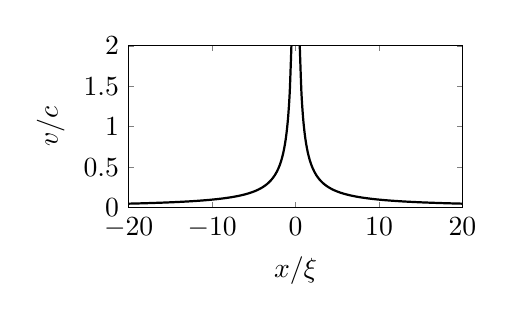
\begin{tikzpicture}
    \begin{axis}[
        width=0.48\linewidth,
        height=0.3\linewidth,
        xlabel=$x/\xi$,
        ylabel=$v/c$,
        xmin=-20,
        xmax=20.0,
        ymax=2,
        ymin=0,
        major tick length = 0.07cm
      ]
      \addplot[mark=none,color=black,thick,domain=0.5:20.0,smooth,samples=100] {1/sqrt(x*x)};
      \addplot[mark=none,color=black,thick,domain=-20.0:-0.5,smooth,samples=100] {1/sqrt(x*x)};
    \end{axis}
  \end{tikzpicture}
  \caption{(a) A comparison of the true vortex solution (black solid line) at $x=0$, found by numerically propagating the GPE in imaginary time, and the Pad\'e approximation (red dashed line) for a vortex core with a charge of $n=1$. (b) Fluid velocity in the vicinity of a vortex at $x=0$ with charge $n=1$.}\label{fig_vortex}
 \end{figure}

As seen in Section \ref{section:hydrodynamic}, the velocity of the fluid can be written $\mathbf{v} = \frac{h}{m}\nabla\theta$, where $\theta$ is the phase. We can use this with Equation \ref{eq_vortexsol} to find the velocity of the fluid around a vortex,
	\begin{equation}\label{eq_vortexvel}
	\mathbf{v}(r,\varphi) = \frac{n \hbar}{mr} {\bm{\hat{\varphi}}},
	\end{equation}
where ${\bm{\hat{\varphi}}}$ is the azimuthal unit vector. Note the $v \propto 1/r$ dependence in the speed of the fluid around the vortex, demonstrated in Figure \ref{fig_vortex} (b). 

\section{\label{section:inital} Initial conditions}
	When numerically solving the GPE, an initial condition must be chosen. Correct choice of initial condition is important for accurate simulation of dynamics. If an unstable initial condition is chosen far from the ground state solution, noise and other excitations such as solitary waves and vortices may be generated that interfere with any measurements and studies undertaken at later times in the numerical computation. A selection of appropriate non-violent initial conditions are outlined in this section. 
	\subsection{\label{section:homoinit} Homogeneous initial condition}
	When the potential term $V=0$, the condensate ground state becomes homogeneous with density $\rho=\mu/g$. In this case, a stationary solution of the GPE is as simple as setting the ground state density everywhere,
	\begin{equation}
		\psi = \sqrt{\frac{\mu}{g}}.
		\label{eq:homoinit}
	\end{equation}

	\subsection{\label{section:tftrap} Thomas-Fermi profile of a trapped condensate}
	Consider an initial condition that is stationary in time, but has a non-zero potential and so varies in space. Such a condition will necessarily satisfy \ref{eq:stationgpe}, the time-independent GPE. Let us assume that we have a strongly repulsive interaction term ($g \gg 0$) and that the potential varies slowly in space. In this case, as an approximation we can neglect the kinetic energy term in the solution as $\nabla^2\psi$ will be negligible compared to the strength of the repulsive atom-atom interactions. We write
	\begin{equation}
		\mu\psi({\bf r}) = \left(V({\bf r}) + g|\psi({\bf r})|^2  \right) \psi({\bf r}),
	\end{equation}
	which can be simplified as,
	\begin{equation}
	 |\psi({\bf r})|^2=\frac{\mu - V({\bf r})}{g}.
	\end{equation}
	From this result, we then construct an approximate solution,
	\begin{equation}
	\psi({\bf r}) =
	\begin{cases} 
    \sqrt{\frac{\mu - V({\bf r})}{g}} & \mathrm{if}~\mu\geq V({\bf r}), \\
    0 & \mathrm{otherwise}.
  \end{cases}
  \end{equation}
	This is known as the Thomas-Fermi (TF) profile and is extremely useful as an approximate initial condition for modelling a trapped atomic condensate. In the case of a harmonic trap, the approximation is accurate near the centre of the condensate but fails near the condensate edge, where the tails of the true density distribution are not captured. Nevertheless Figure \ref{fig_tfprofile} demonstrates the high accuracy of the approximation. Due to the discrepancy at the tails of the condensate density, it is often the case that the TF profile is used as an initial guess for numerical eigensolvers, which then find a time-independent numerical solution to be used as the true initial condition.
	\begin{figure}
	\centering
   \begin{tikzpicture}
    \begin{axis}[
        width=0.58\linewidth,
        height=0.3\linewidth,
        xlabel=$x/l_r$,
        ylabel=$|\tilde{\psi}|^2$,
        xmin=-20,
        xmax=20,
        ymin=0,
        major tick length = 0.07cm
      ]
      \addplot gnuplot [raw gnuplot,mark=none,color=black,thick]{
      	plot "numerics/figures/TF.dat" using 1:2 with lines;
      };
      \addplot gnuplot [raw gnuplot,mark=none,color=red,thick,dashed]{
      	plot "numerics/figures/TF.dat" using 1:3 with lines;
      };
    \end{axis}
  \end{tikzpicture}
  \begin{tikzpicture}
    \begin{axis}[
        width=0.38\linewidth,
        height=0.3\linewidth,
        xlabel=$x/l_r$,
        ylabel={},
        xmin=6,
        xmax=8.5,
        major tick length = 0.07cm
      ]
      \addplot gnuplot [raw gnuplot,mark=none,color=black,thick,smooth]{
      	plot "numerics/figures/TF.dat" using 1:2 with lines;
      };
      %\addplot gnuplot [raw gnuplot,mark=none,color=green,thick,dashed,samples=100]{
      	%plot "numerics/figures/TF.dat" using 1:3 with lines;
      %};
      \addplot[mark=none,color=red,dashed,thick,domain=6:7.11,smooth,samples=100] {(25.26698674-0.5*x*x)/2000.0};
      \addplot[mark=none,color=red,dashed,thick,domain=7.11:9,smooth,samples=100] {0.0*x};
    \end{axis}
  \end{tikzpicture}
  \caption{Comparison of the TF profile (red dashed line) and the true trapped ground state (black solid line) for a condensate in a harmonic trap, as found by numerical solution of the GPE in imaginary time. The TF profile fits extremely well over most of the condensate density (left), however fails at capturing the smooth tails of the density distribution (right). Here the TF radius is approximately $R_{\mathrm{TF}} = 7.1\,l_r$ and can be identified as a kink in the TF profile.}\label{fig_tfprofile}
 \end{figure}

 The TF solution provides a useful analytic approximation for the size of a condensate. The perimeter of the fluid occurs approximately when $\mu = V({\bf r})$, and so the approximate Thomas-Fermi radius of the condensate is,
	\begin{equation}
	R_{\mathrm{TF}} = \sqrt{\frac{2\mu}{m\omega_r^2}}.
	\end{equation}
The TF radius is a useful indicator of length scales when working with analytical descriptions of condensate behaviours in a trapped system.

\subsection{\label{section:cfieldinitcond} Classical field initial condition}
	In numerical simulation of a finite temperature Bose gas, we begin with a highly non-equilibrium state, so that the low-lying coherent modes of the system are all highly occupied. The corresponding initial condition is
	\begin{equation}
	\psi_{\rm neq}({\bf r}) = \sum \limits_{\bf k}^{k<k_{\rm max}} a_{\bf k} \exp (\mathrm{i}{\bf k}\cdot{\bf r}),
	\label{eq:cFieldIC}
	\end{equation}
	where the complex Fourier amplitudes $a_{\bf k}$ are related to the occupation numbers $n_{\bf k}$ through $\braket{a_{\bf k}^{\,}a_{\bf k'}^*} = n_{\bf k}\delta_{\bf kk'}$. The phase of the complex amplitudes $a_{\bf k}$ are distributed uniformly on $[0,2\pi]$ while $|a_{\bf k}|$ is distributed randomly with fixed mean equal to unity; it has been found that different distributions of $|a_{\bf k}|$ make no qualitative difference to the turbulent evolution \cite{PhysRevA.66.013603}. A momentum cutoff, $k<k_{\rm max}$, is introduced to limit the momentum of the low lying modes, and in harmonic systems can be imposed as an energy-cutoff during evolution using the projected GPE \cite{PhysRevLett.87.160402}. However, in the case of homogeneous finite temperature simulations the momentum cut-off arises naturally as a consequence of the discretisation of the system; for a 3D finite temperature simulation in a periodic box with uniform grid spacing $\Delta$, $k_{\rm max}=\sqrt{3} \pi / \Delta$.

	The numerical initial condition $\psi({\bf r},t_0)$ is then determined by renormalisation of $\psi_{\rm neq}({\bf r})$ to fix the number density, $N/V$ and kinetic energy density, $E_{\rm kin}/V$. The choice of $N/V$ and $E_{\rm kin}/V$ uniquely determines the condensate fraction, and therefore the temperature for the equilibrium state of the Bose gas.

\section{\label{section:potentials}Modelling obstacles and surfaces}
In atomic BEC experiments, adding obstacles can be achieved by using laser beams. A red-detuned laser beam can create areas of attraction, and conversely, blue-detuned laser beams can create areas of repulsion. Should a blue-detuned laser beam be bright enough, a localised `hole' in the condensate forms. Similarly, in superfluid helium experiments, there are examples where the fluid can feel the presence of obstacles, including grids \cite{Davis2000,brad05}, wires \cite{Guenault1986,Bradley2011,Fisher2001}, forks \cite{Blaauwgeers2007,Bradley2012}, propellers \cite{Tabeling,Salort}, spheres \cite{Schoepe1995} and other objects \cite{VinenSkrbek2008}.

These effects are replicated in the GPE model through the use of two and three-dimensional potentials. In atomic BEC simulations the profile of the potential matches that of the intensity of the laser beam, typically a cylindrical beam with a Gaussian profile. In superfluid helium simulations, smooth or hard wall potentials are used with an amplitude large compared to the chemical potential.
\subsection{\label{section:3dobjpotential} Three-dimensional elliptical Gaussian}
In our 3D simulations the localized obstacle is modelled via a repulsive Gaussian potential,
\begin{equation}
V_{\mathrm{obj}}({\bf r})=V_0 \exp \left( -\frac{\varepsilon^2(x-x_0)^2}{d^2} -\frac{(y-y_0)^2}{d^2}-\frac{(z-z_0)^2}{d^2}\right),
\label{eq:potential3D}
\end{equation}
where  $V_0$ is its amplitude, $d$ its width in the $y$ and $z$ directions, and $(x_0,y_0,z_0)$ its coordinates. $\varepsilon$ parametrises the ellipticity of the obstacle, a value of $\varepsilon=1$ corresponds to a spherical obstacle, a higher value of $\varepsilon$ `squashes' the obstacle along $x$, forming a pancake shape.

\subsection{\label{section:3dcylinderpotential} Two and three-dimensional cylindrical Gaussian}
In addition to spheres, we model cylindrical potentials as a Gaussian,
\begin{equation}
V_{\mathrm{obj}}({\bf r})=V_0 \exp \left( -\frac{\varepsilon^2(x-x_0)^2}{d^2} -\frac{(y-y_0)^2}{d^2}\right),
\label{eq:potentialcylinder}
\end{equation}
where  $V_0$ is its amplitude, $d$ its width in the $y$ direction, and $(x_0,y_0)$ its coordinates. $\varepsilon$ parametrises the ellipticity of the Gaussian (experimentally feasible with laser beam focusing or masking), so that a value of $\varepsilon=1$ corresponds to a circular shaped hole. In 3D the Gaussian hole is extended across the entire $z$ dimension forming a cylindrical shaped barrier.
\subsection{\label{section:3dafmpotential} Three-dimensional `realistic' rough-surface}
\begin{figure}
	\centering
  \begin{tikzpicture}
    \begin{axis}[
        width=0.5\linewidth,
        xlabel={$x$ ($\mu$m)},
        ylabel={$y$ ($\mu$m)},
        xmin=-0.5,
        xmax=0.5,
        ymin=-0.5,
        ymax=0.5,
        major tick length = 0.07cm,
        axis on top,
        unit vector ratio=1 1 1,
        axis on top,
        colorbar style={title={\makebox[\linewidth]{z (nm)}},text width=0.5em,major tick length = 0.07cm},
        major tick length = 0.07cm,
        point meta min = 0,
        point meta max = 16,
        colorbar,colormap/jet
      ]
      \addplot graphics [xmin=-0.5,xmax=0.5,ymin=-0.5,ymax=0.5] {afm/afm2.png};
    \end{axis}
  \end{tikzpicture}
  \caption{An atomic force microscope (AFM) image showing the microscopic detail on the surface of a  single--core NbTi `floppy' wire used for generating superfluid turbulence. This data was kindly provided by C. R. Lawson \cite{Lawson}.}\label{fig_afmprofile}
 \end{figure}

In many superfluid helium experiments \cite{VinenSkrbek2008} turbulence is generated by moving obstacles, the surface of which are rough on the length scale of the superfluid vortex core, which is of
the order of $10^{-10}~\rm m$ in $^4$He
and $10^{-8}~\rm m$ in $^3$He.  As an example, Figure \ref{fig_afmprofile} is an atomic force microscope (AFM) image showing the microscopic detail on the surface of a  single--core NbTi `floppy' wire used for generating superfluid turbulence  \cite{Bradley2011}.  Note the appearance of an elongated scratch, believed to be typical of such wires.

We can simulate the microscopic detail through the use of a potential derived from sample AFM height-map data. We define the external potential to be,
\begin{equation}
V_{\mathrm{obj}}({\bf r}) =
\begin{cases}
V_0 &\mbox{if } z < (h(\alpha x,\alpha y)-z_0)  \\
0 &\mbox{if } z > (h(\alpha x,\alpha y)-z_0),
\end{cases}
\label{eq:potentialAFM3D}
\end{equation}
where $V_0$ is its amplitude, $z_0$ is a shift in height and $\alpha$ is a lateral scaling factor. Scaling $h(x,y)$ acts as a crude way of varying the roughness of simulated boundaries. Finally, a Gaussian blur is applied to the raw AFM data so that $V(x,y,z)$ is smooth.

\end{chapter}
